\documentclass[11pt]{article}
\usepackage{graphicx}
\usepackage{multirow}
\usepackage{float}
\usepackage{hyperref}
\usepackage{biblatex}
\usepackage{algpseudocode}

\graphicspath{ {../img/} }
\addbibresource{cite.bib}

\renewcommand{\figurename}{Slika}
\renewcommand{\tablename}{Tabela}
\renewcommand{\contentsname}{Kazalo}
\renewcommand{\contentsname}{Kazalo}
\renewcommand{\listfigurename}{Kazalo slik}
\renewcommand{\listtablename}{Kazalo tabel}

\title{Stiskanje slik s pomočjo razvrščanja z voditelji \\ {\small Projektna naloga pri predmetu Vzporedni in porazdeljeni sistemi in algoritmi}}

\date{2022 \\ Januar}
\author{Nik Prinčič \\[1cm]{\small Mentorji: izr. prof. dr. Patricio Bulić, as. Davor Sluga, as. Rok Češnovar}}
\begin{document}
\maketitle

\newpage

\tableofcontents
\newpage
\listoffigures
\listoftables

\newpage

\section{Motivacija}
Stiskanje slik je postopek, ki s pomočjo različnih tehnik, zmanjša velikost slike.
Poznamo več različnih načinov stiskanja, delimo jih na brezizgubne (angl. lossless) in izgubne (angl. lossy).
Stiskanje s pomočjo razvrščanja z voditelji spada med transformacijske metode, ki sodijo med izgubne načine kompresije.


\section{Opis algoritma}
\label{sec:algorithm}
Algoritem deluje po principu razvrščanja z voditelji.

\begin{enumerate}
    \item Izberemo število gruč (k) in število iteracij (n)
    \item Vsaki gruči dodelimo naključen slikovni element
    \item Za vsak slikovni element izračunam razdaljo do najbližje gruče (uporabimo evklidsko razdaljo) in ga dodelimo tej gruči
    \item Za vsako gručo izračunamo povprečno barvo vseh pripadajočih slikovnih elementov,
          ta povprečna barva prestavlja centroido gruče. Če gruči ne pripada noben slikovni element ji priredimo naključnega.
    \item 3. in 4. korak ponovimo n-krat
    \item Izhodno sliko sestavimo tako, da vsakemu slikovnemu elementu priredimo barvo pripadajoče gruče
\end{enumerate}


\section{Implementacije algoritma}

\subsection{Serijska implementacija}
Serijski algoritem je implementiran v jeziku C. Za branje in shranjevanje slike je bila uporabljena knjižnica FreeImage\cite{FreeImage}.
Vhod v algoritem je slika prebrana s pomočjo knjižnice FreeImage, zapisana je v polju tipa \emph{unsigned char}, 4 zaporedne vrednosti v polju pa predstavljajo en slikovni element v obliki \emph{BGRA}.
Poleg polja kjer je hranjena slika se uporablja še polje v katerem se harnijo vrednosti centroidov gruč,
polje v katerem se za vsak slikovni element hrani indeks gruče kateri pripada,
polje v katerem se hrani število slikovnih elementov, ki pripadajo vsaki gruči,
ter polje, ki deluje kot akumulator (za vsako gručo se seštevajo vrednosti pripadajočih slikovnih elementov).
Postopek izračuna je za seriski algoritem popolnoma enak, kot je opisano v \hyperref[sec:algorithm]{Opis algoritma}

\subsection{Paralelna implementacija na CPE}
Algoritem sem na CPE paraleliziral z uporabo knjižnice OpenMP \cite{OMP}.
OpenMP je aplikacijski programski vmesnik (angl. Application Programming Interface), ki podpira paralelizacijo z deljenim pomnilnikom. Sestavlja ga nabor direktiv za prevajalnik, knjižničnih rutin  in globalnih spremenljivk ki vplivajo na izvajanje programa.
Osnova za paralelno implemenatcijo je serijska implementacija. pred paralelno sekcijo sem dodal klic funkcije, ki nastavi število niti, ki jih bo OpenMP uporabil za izvajanje kode v paralelni sekciji.
Nato pa sem določil katere zanke bom paraleliziral in jim dodal potrebne direktive.
Odločil sem se, da paraleliziram
\begin{itemize}
    \item zanko, ki na začetku gručam dodeli naključne vrednosti. Seveda je ta odločitev pri majhnem številu gruč nesmiselna, pri večjem številu baru pa bi tudi ta del pozitivno vplival na čas izvajanja.
    \item zanko, ki za vsak piksel računa najbižjo gručo in vrednosti slikovnih elementov prišteva v akumulator izbrane gruče.
    \item zanko, ki za vsako gručo izračuna povprečno vrednost pripadajočih slikovnih elementov
    \item zanko, ki v zadnjem koraku izhodni sliki dodeli barve
\end{itemize}

\bigskip\noindent
Pri paralelizaciji druge zanke sem se odločil za sledeči pristop:
vsaka nit dobi svojo privatno akumulatorsko polje v katerega lahko prišteva dobljene vrednosti ter polje za štetje pripadnosti gručam,
nato pa se v kritični sekciji (\emph{\#pragma omp critical}) privatna polja združijo v globalno.
Za ta pristop sem se odločil, potem ko sem najprej prištevanje v akumulatorsko polje izvedel s pomočjo atomičnih operaciji (\emph{\#pragma omp atomic}) in prištevanjem direktno v globalno polje,
a z dobljenimi rezultati nisem bil najbolj zadovoljen.

\bigskip\noindent
Paralelnim delom kode lahko nastavimo tudi način razvrščanja (angl. schedule), izbiramo lahko med \emph{static}, \emph{dynamic} in \emph{guided}, nastavimo pa lahko tudi \emph{chunk size}.
Testiral sem različne kombinacije nastavitev, a najboljše rezulatet sem dobil z privzeto vrednostjo (\emph{schedule(static, iterations / threads)}

\subsection{Paralelna implementacija na GPE}
Algoritem sem na GPE paraleliziral z uporabo knjižnice OpenCL \cite{OpenCL}. OpenCL je ogrodje za pisanje programov, ki se izvajajo na heterogenih sistemih, v tem primeru se program izvaja na grafični procesni enoti.
Osnovni algoritem je bilo potrbno razdeliti v dva ščepca (angl. kernel), v prvem se odvija izračun najbližjih gruč, v drugem pa izračun povprečne barve za vsako gručo, dodal pa sem še tretji ščepec, v katerem se barve gruč aplicirajo na izhodno sliko. Za uporabo tretjega ščepca sem se odločil,
saj so vsi potrebni podatki že prisotni na GPE in tako za zagon še enega ščepca ne plačamo nobene časovne kazni.
Dodal sem tudi uporabo lokalnega pomnilnika v obeh ščepcih. Velikost delovne skupine sem v prvem ščepcu nastavil na 16 * 16 (uporabil sem dvodimenzijonalno obliko ščepca), v drugem ščepcu pa sem velikost delovne skupine nastavil na 16 (uporabil sem enodimenzijonalno obliko ščepca).

\bigskip\noindent
Prvi ščepec si v lokalni pomnilnik prenese centroide gruč ter vhodno sliko, saj do teh dveh podatkov največkrat dostopa.
Drugi ščepec pa si v lokalni pomnilnik prenese akumulatorsko polje barve gruč, ki se je napolnilo v prvem ščepcu.


\section{Rezultati}
Algoritem sem testiral na eni sliki, ki je podana v osmih različnih dimenzijah. Najmanjša je velikosti 320x240, največja pa 6016x3384.
Vse teste sem izvedel dvakrat in izračunal povprečje.

\bigskip\noindent
Vse teste sem izvdele pri 50 iteracijah in vrednostih parametra \emph{k} (število gruč) 16, 32, 64, 128 in 256.
Pri paralelni različici na CPE sem te teste ponovil pri različnem številu niti (2, 4, 8, 16, 32 in 64)

\bigskip\noindent


\begin{figure}[H]
    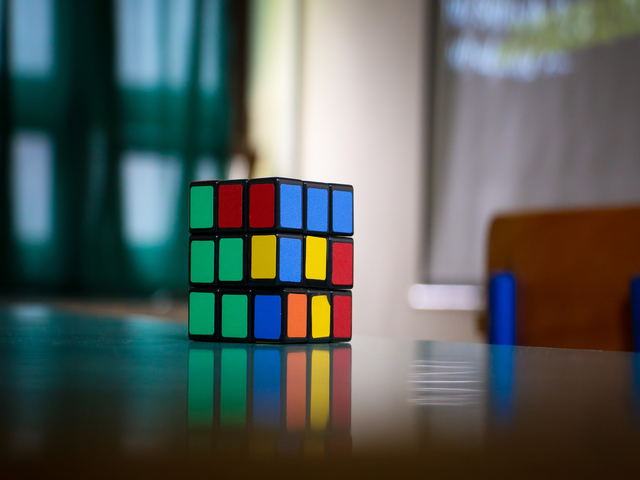
\includegraphics[scale=0.4]{cube_640x480}
    \centering
    \caption{Slika uporabljena za testiranje}
\end{figure}



\subsection{Rezultat kompresije}
Slika 2 predstavlja rezultat kompresije pri parametrih \emph{k}=64 in \emph{n}=50 (\emph{k}—število gruč, \emph{n}—število iteracij), slika 3 pa rezultat po kompresiji z parametri \emph{k}=32 in \emph{n}=50.

\begin{figure}[H]
    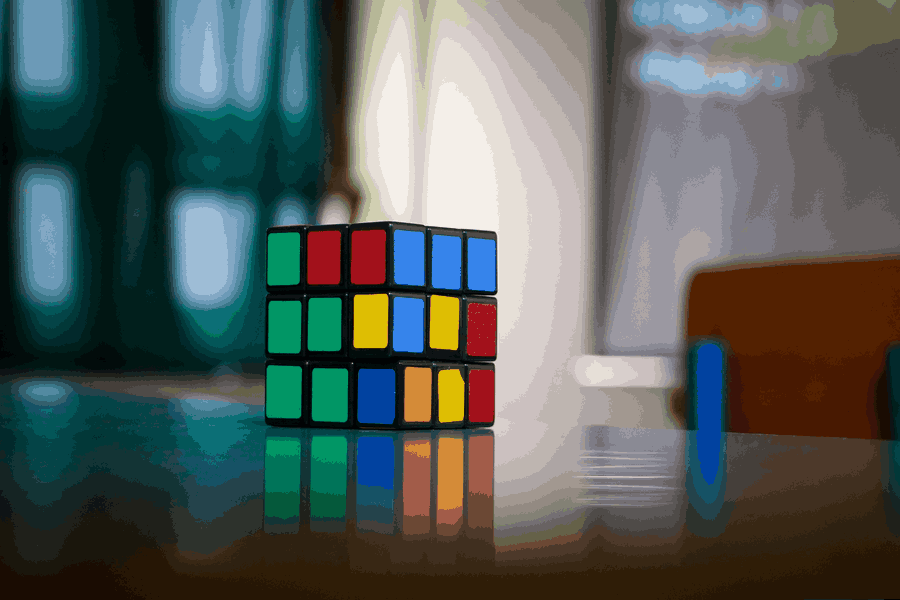
\includegraphics[scale=0.2]{out_64}
    \centering
    \caption{Rezultat kompresije pri parametri k=64 in n=50}
\end{figure}

\begin{figure}[H]
    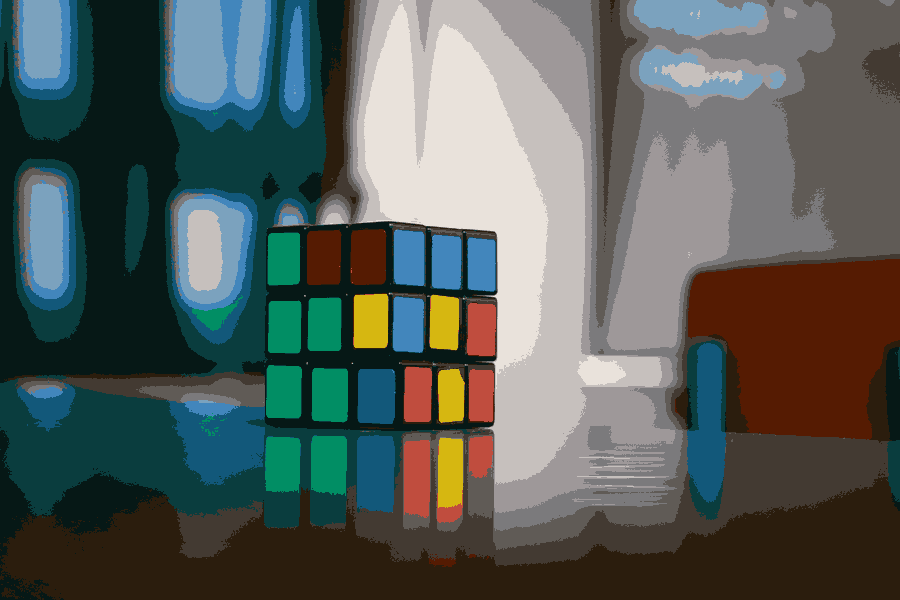
\includegraphics[scale=0.2]{out_16}
    \centering
    \caption{Rezultat kompresije pri parametri k=16 in n=50}
\end{figure}

\subsubsection{Primerjava učinkovitosti kompresije}
\begin{table}[h]
    \centering
    \begin{tabular}{l | l | l}
        kompresija & Velikost [KB] & Relativna velikost [\%] \\
        \hline
        brez       & 574           & 100                     \\
        \hline
        k=64       & 104           & 18                      \\
        \hline
        k=16       & 41            & 7                       \\
    \end{tabular}
    \caption{Primerjava učinkovitosti kompresije}
\end{table}

\subsection{Primerjava časa izvjanaj}

Za paralelno različico na GPE in CPE sem izračunal tudi pohitritev po formuli $S=t_s/t_p$, kjer $t_s$ predstavlja čas izvajanja serijskega programa, $t_s$ pa čas izvajanja paralelnega programa.
Za paralelno različico na CPE pa sem izračunal tudi učinkovitost paralelizacije po formuli $E=S/p$ kjer $p$ predstavlja število niti, ki jih je uporabil paralelni program.


\subsubsection{Čas izvajanja serijskega algoritma}
\begin{figure}[H]
    \label{img:cpu}
    \centering
    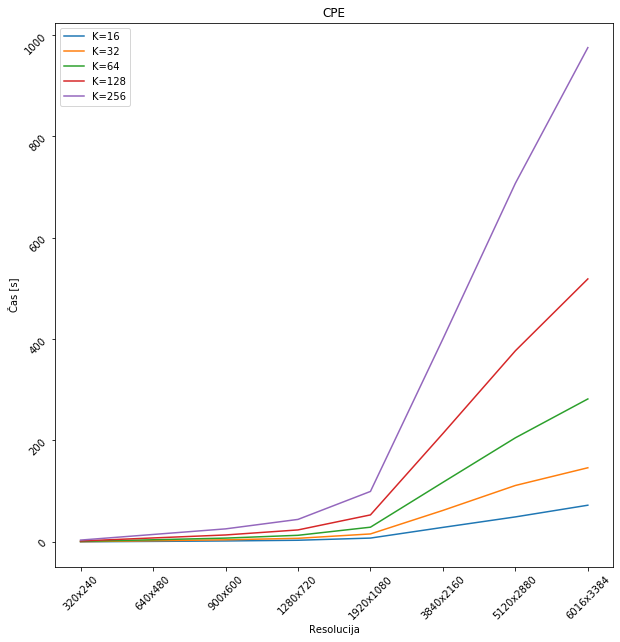
\includegraphics[scale=0.5]{cpu}
    \caption{Izmerjeni časi izvajanja serijske implmentacije algoritma}
\end{figure}
Iz grafa lahko opazimo da se čas izvajanja ne povečuje linearno.
Podrobni podatki meritev so dostopni v \hyperref[dat:cpu]{Tabela 2}.


\subsubsection{Čas izvajanja paralelnega algoritma na CPE}
\begin{figure}[H]
    \label{img:cpup}
    \centering
    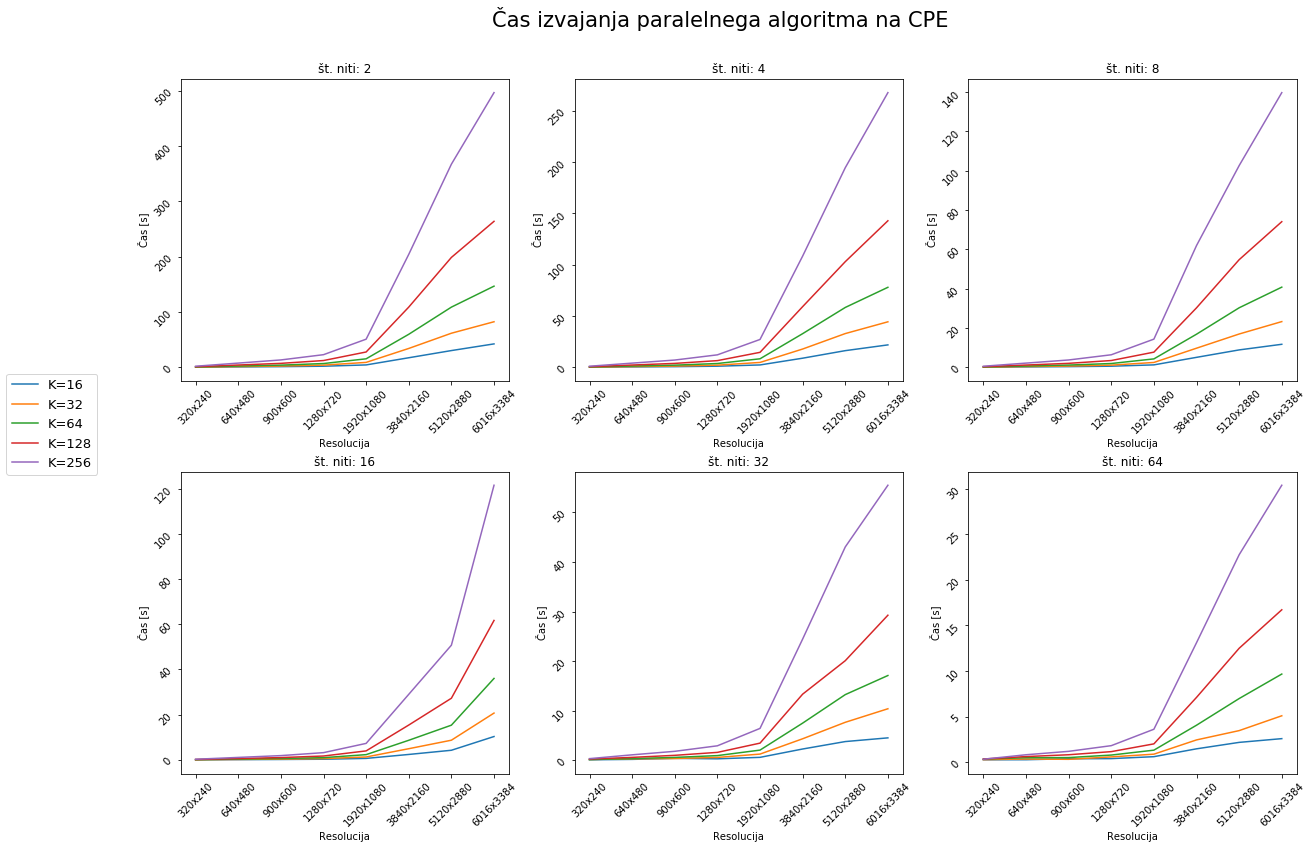
\includegraphics[scale=0.3]{cpup}
    \caption{Izmerjeni časi izvajanja paralelne implementacija algoritma na CPE}
\end{figure}

Pri paralelni implementaciji na CPE, lahko opazimo,
da čas izvajanja narašča podobno hitro kot pri serijski implementaciji.
Podrobni podatki meritev so dostopni v \hyperref[dat:cpup]{Tabela 3}.


\subsubsection{Čas izvajanja paralelnega algoritma na GPE}
\begin{figure}[H]
    \label{img:gpu}
    \centering
    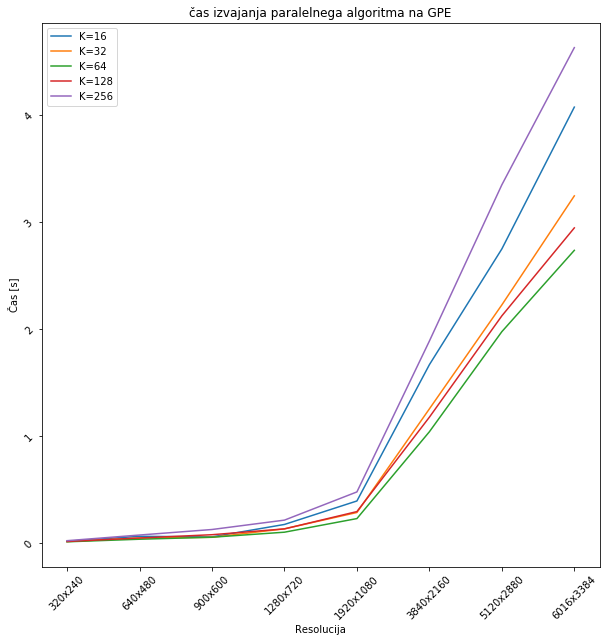
\includegraphics[scale=0.5]{gpu}
    \caption{Izmerjeni časi izvajanja paralelne implementacija algoritma na GPE}
\end{figure}

Pri tej različici algoritma, lahko opazimo ogromno pohitritev, kar je bilo tudi pričakovano.
Podobno kot pri paralelni različici na CPE tudi tukaj da čas izvajanja ne narašča linearno, zanimivo pa je tudi, da primer ko uporabimo $k=64$ izvede najhitreje.
Podrobni podatki meritev so dostopni v \hyperref[dat:gpu]{Tabela 4}.

\subsubsection{Pohitritev paralelnega algoritma na CPE}
\begin{figure}[H]
    \label{img:cpup_perf}
    \centering
    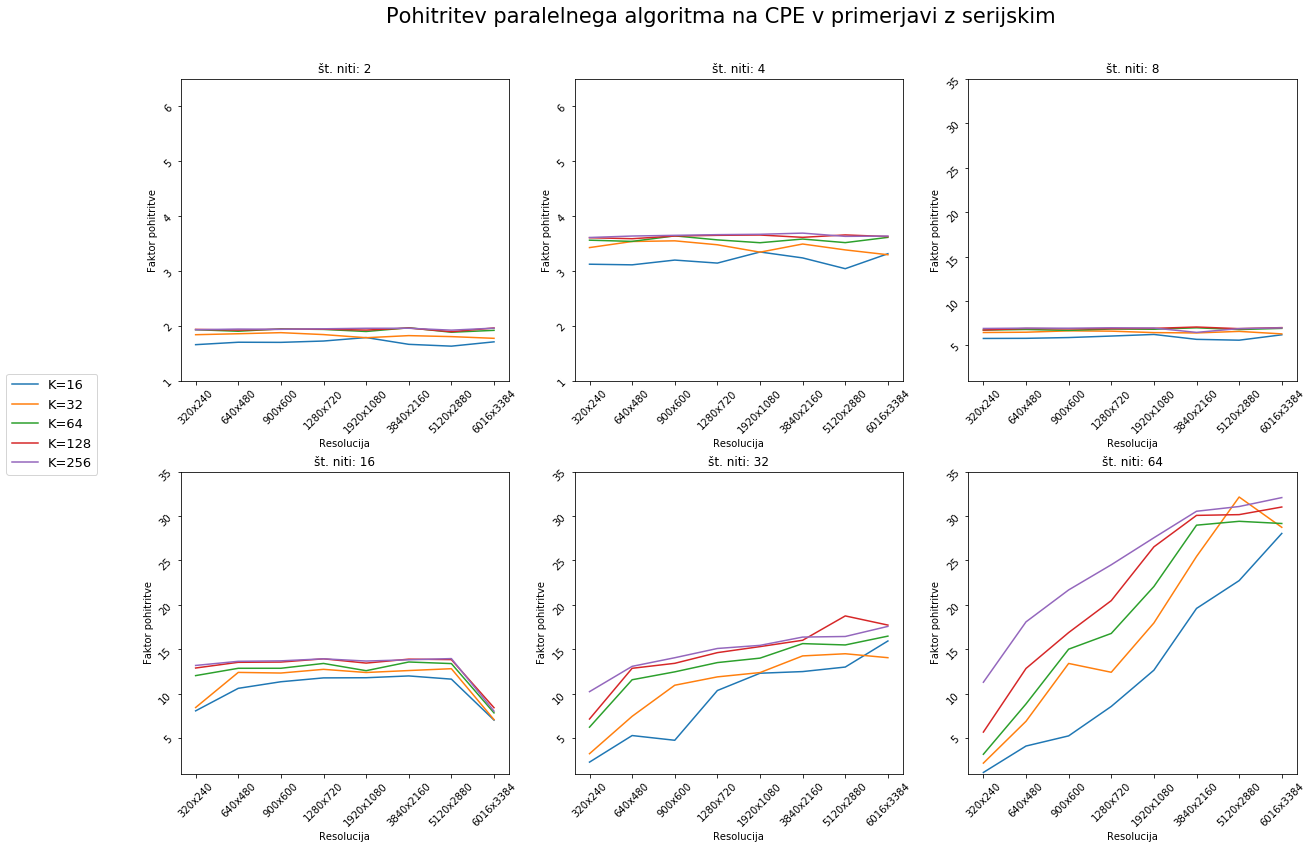
\includegraphics[scale=0.28]{cpup_perf.png}
    \caption{Pohitritev paralelnega algoritma na CPE v primerjavi z serijskim}
\end{figure}

Iz grafa lahko razberemo, da je pri številu uporabljenih niti med 2 in 16 pohitritev dokaj neodvisna od velikosti vhodne slike in števila gruč,
pri uporabi 32 in 64 niti pa pohitritev narašča z narščanjem velikosti vhodne slike.

\subsubsection{Učinkovitost paralelizacije algoritma na CPE}
\begin{figure}[H]
    \label{img:cpup_eff}
    \centering
    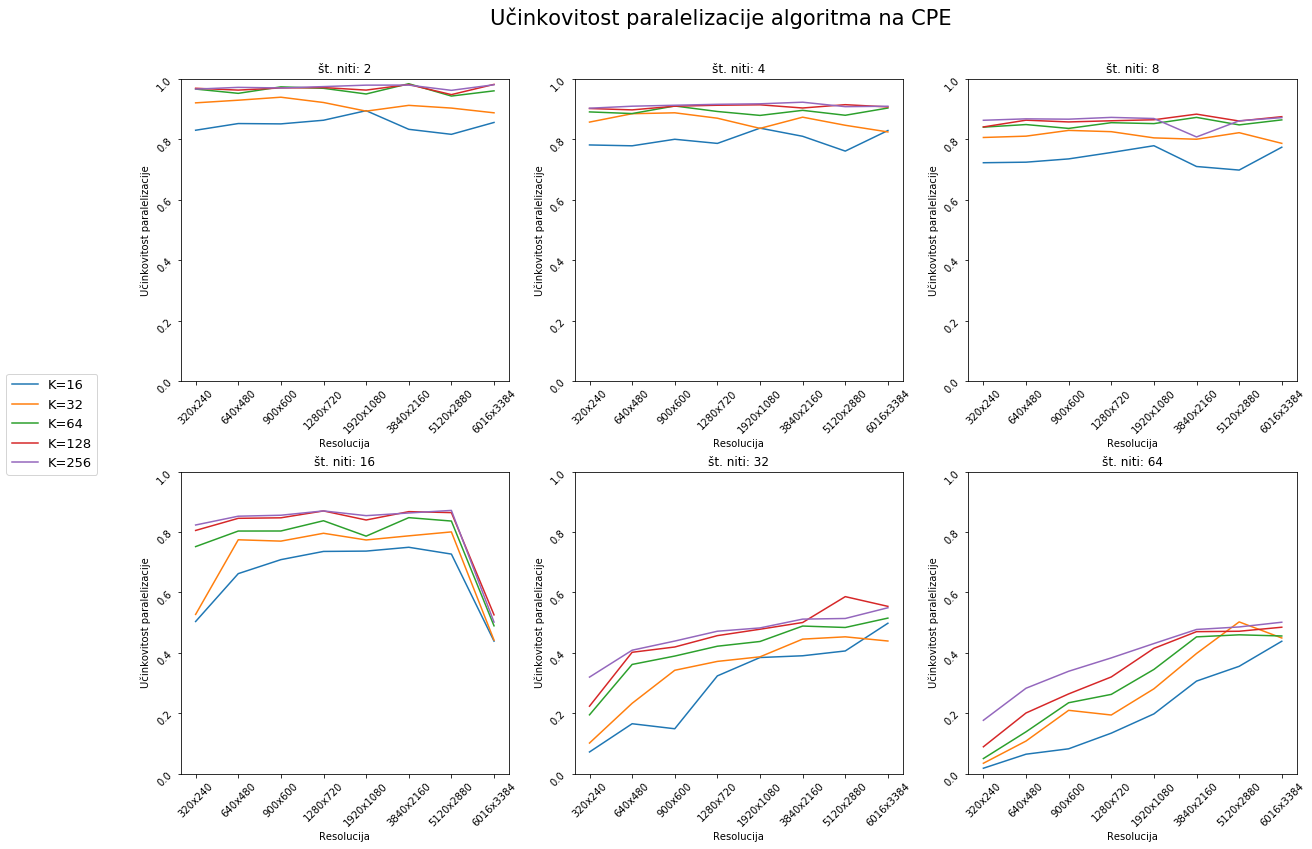
\includegraphics[scale=0.28]{cpup_eff.png}
    \caption{Učinkovitost paralelizacije algoritma na CPE}
\end{figure}

Iz grafa lahko razberemo, da je učinkovitost paralelizacije najvišja ko uporabimo med 2 in 8 niti,
pri uporabi 32 in 64 niti pa učinkovitost paralelizacije narašča z večanjem vhodne slike, a nikoli ne preseže 60\%.

\begin{figure}[H]
    \label{img:thread_comp}
    \centering
    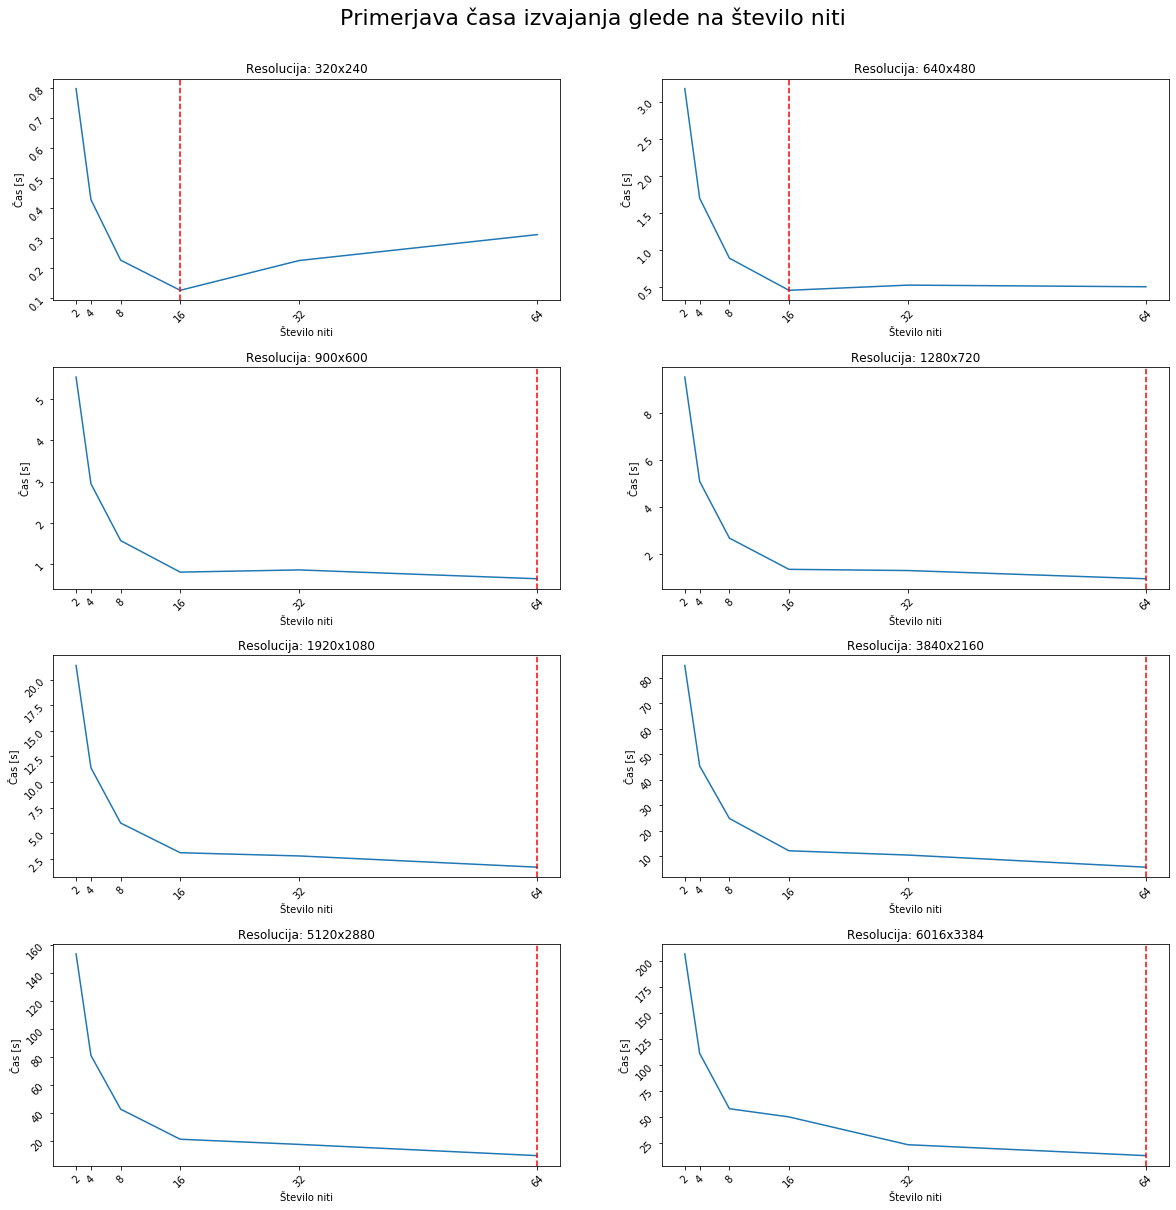
\includegraphics[scale=0.28]{thread_comp.png}
    \caption{Primerjava časa izvajanja paralelnega algoritma na CPE glede na število uporabljenih niti}
\end{figure}

\bigskip\noindent
Iz grafa lahko razberemo, da je pri manjših velikostih vhodne slike bolj smiselno uporabiti manjše število niti,
pri večjih vhodnih slikah pa nam dodatne niti pripomorejo k krajšemu času izvajanja.


\subsubsection{Pohitritev paralelnega algoritma na GPE}
\begin{figure}[H]
    \label{img:gpu_perf}
    \centering
    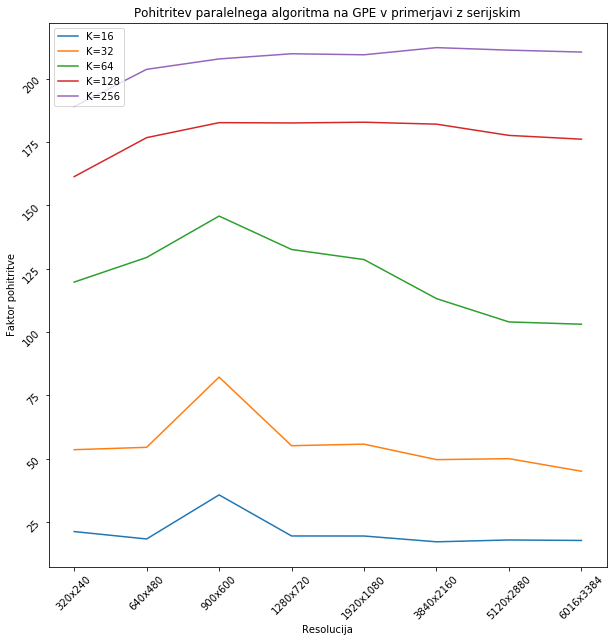
\includegraphics[scale=0.28]{gpu_perf.png}
    \caption{Pohitritev paralelnega algoritma na GPE v primerjavi z serijskim}
\end{figure}

Kot je bilo pričakovati je pohitritev na GPE daleč največja, nanjo pa zelo vpliva izbira števila gruč.

\subsection{Primerjava vseh implementacij algoritmov}
\begin{figure}[H]
    \label{img:comp}
    \centering
    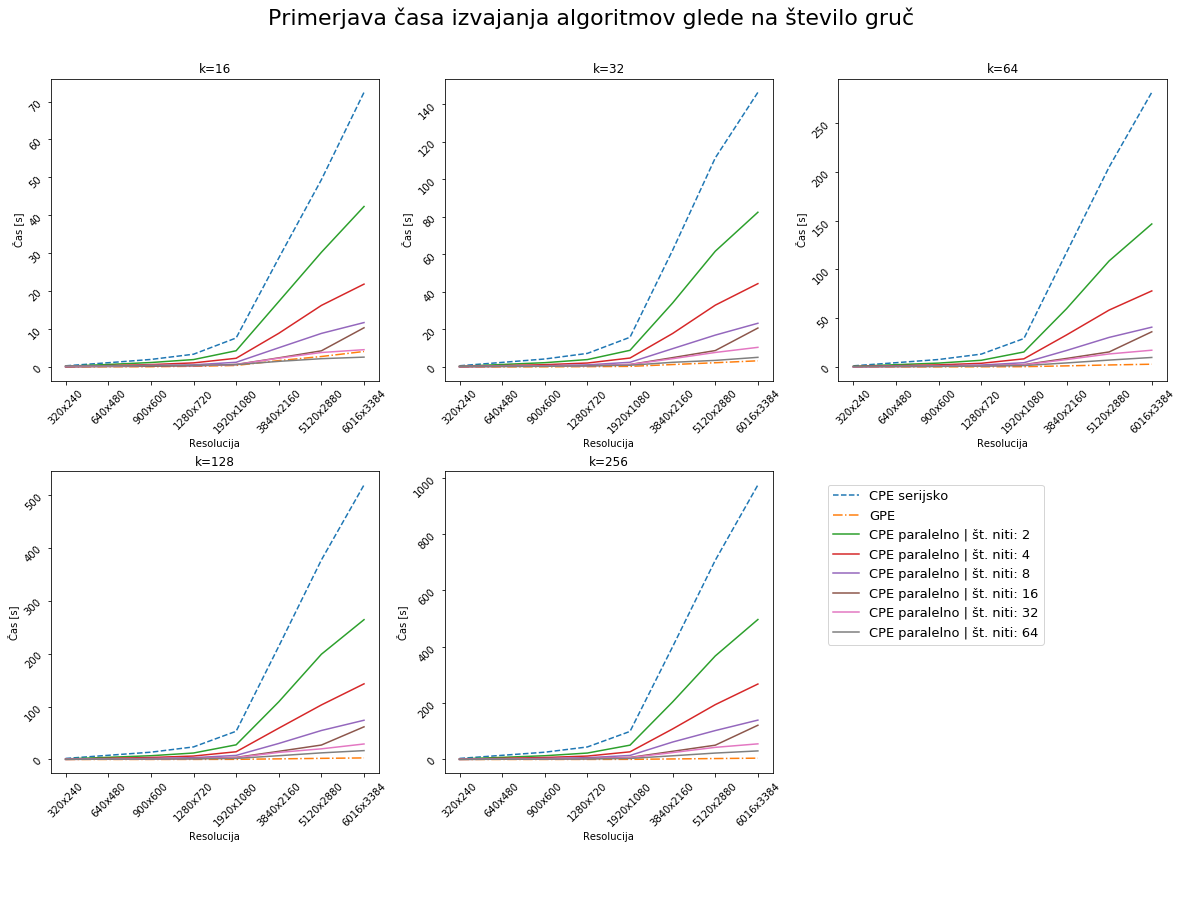
\includegraphics[scale=0.28]{comp.png}
    \caption{Primerjava vse implementaciji algoritmov}
\end{figure}

Iz zgornjega grafa lahko razberemo da je GPE v večini primerov najboljša izbira, razen pri vrednosti parametra $k$ 16 in 32, tu je paralelna implementacija na CPE enakovredna ali celo hitrejša.
Serijska implementacija je kot je bilo pričakovano najpočasnejša.

\section{Zaključek}
Pri implementaciji algoritmov nisem imel pretiranih težav, vsekakor pa bi se vse tri implmentacije dalo še dodatno optimizirati in izpopolniti.
Dobljeni rezultati so v skladu z začetnimi pričakovanji, nekatera manjša odstopanja bi lahko odpravil z večimi ponovitvami testa.

\begin{table}[H]
    \centering
    \label{dat:cpu}
    \begin{tabular}{c|c|c|c|c}
        $k$ & $n$ & $width$ & $height$ & $time$     \\
        \hline
        16  & 50  & 320     & 240      & 0.294847   \\
        16  & 50  & 640     & 480      & 1.108794   \\
        16  & 50  & 900     & 600      & 1.973933   \\
        16  & 50  & 1280    & 720      & 3.349446   \\
        16  & 50  & 1920    & 1080     & 7.634581   \\
        16  & 50  & 3840    & 2160     & 28.719472  \\
        16  & 50  & 5120    & 2880     & 49.373230  \\
        16  & 50  & 6016    & 3384     & 72.419973  \\
        32  & 50  & 320     & 240      & 0.603921   \\
        32  & 50  & 640     & 480      & 2.397267   \\
        32  & 50  & 900     & 600      & 4.208989   \\
        32  & 50  & 1280    & 720      & 7.191427   \\
        32  & 50  & 1920    & 1080     & 15.787287  \\
        32  & 50  & 3840    & 2160     & 62.176949  \\
        32  & 50  & 5120    & 2880     & 111.323453 \\
        32  & 50  & 6016    & 3384     & 146.253363 \\
        64  & 50  & 320     & 240      & 1.088703   \\
        64  & 50  & 640     & 480      & 4.300878   \\
        64  & 50  & 900     & 600      & 7.574608   \\
        64  & 50  & 1280    & 720      & 13.112517  \\
        64  & 50  & 1920    & 1080     & 29.095130  \\
        64  & 50  & 3840    & 2160     & 117.500101 \\
        64  & 50  & 5120    & 2880     & 205.284920 \\
        64  & 50  & 6016    & 3384     & 281.894440 \\
        128 & 50  & 320     & 240      & 1.972494   \\
        128 & 50  & 640     & 480      & 7.892978   \\
        128 & 50  & 900     & 600      & 13.769792  \\
        128 & 50  & 1280    & 720      & 23.701236  \\
        128 & 50  & 1920    & 1080     & 53.306609  \\
        128 & 50  & 3840    & 2160     & 213.752218 \\
        128 & 50  & 5120    & 2880     & 376.831908 \\
        128 & 50  & 6016    & 3384     & 518.497545 \\
        256 & 50  & 320     & 240      & 3.690027   \\
        256 & 50  & 640     & 480      & 14.744494  \\
        256 & 50  & 900     & 600      & 25.778977  \\
        256 & 50  & 1280    & 720      & 44.433600  \\
        256 & 50  & 1920    & 1080     & 99.583465  \\
        256 & 50  & 3840    & 2160     & 400.276795 \\
        256 & 50  & 5120    & 2880     & 707.024048 \\
        256 & 50  & 6016    & 3384     & 974.444850 \\
    \end{tabular}
    \caption{Izmerjeni časi za serijski algoritem}
\end{table}

\begin{table}[H]
    \centering
    \label{dat:cpup}
    \begin{tabular}{c|c|c|c|c|c}
        $k$ & $n$ & $t$ & $width$ & $height$ & $time$     \\
        \hline
        16  & 50  & 2   & 6016    & 3384     & 42.311170  \\
        16  & 50  & 4   & 6016    & 3384     & 21.837430  \\
        16  & 50  & 8   & 6016    & 3384     & 11.698559  \\
        16  & 50  & 16  & 6016    & 3384     & 10.325713  \\
        16  & 50  & 32  & 6016    & 3384     & 4.548478   \\
        16  & 50  & 64  & 6016    & 3384     & 2.583756   \\
        32  & 50  & 2   & 6016    & 3384     & 82.374052  \\
        32  & 50  & 4   & 6016    & 3384     & 44.349629  \\
        32  & 50  & 8   & 6016    & 3384     & 23.240360  \\
        32  & 50  & 16  & 6016    & 3384     & 20.699447  \\
        32  & 50  & 32  & 6016    & 3384     & 10.417131  \\
        32  & 50  & 64  & 6016    & 3384     & 5.092522   \\
        64  & 50  & 2   & 6016    & 3384     & 146.743476 \\
        64  & 50  & 4   & 6016    & 3384     & 77.993739  \\
        64  & 50  & 8   & 6016    & 3384     & 40.768459  \\
        64  & 50  & 16  & 6016    & 3384     & 36.027144  \\
        64  & 50  & 32  & 6016    & 3384     & 17.118555  \\
        64  & 50  & 64  & 6016    & 3384     & 9.671210   \\
        128 & 50  & 2   & 6016    & 3384     & 264.031157 \\
        128 & 50  & 4   & 6016    & 3384     & 142.877569 \\
        128 & 50  & 8   & 6016    & 3384     & 74.075239  \\
        128 & 50  & 16  & 6016    & 3384     & 61.678454  \\
        128 & 50  & 32  & 6016    & 3384     & 29.275641  \\
        128 & 50  & 64  & 6016    & 3384     & 16.724037  \\
        256 & 50  & 2   & 6016    & 3384     & 496.833751 \\
        256 & 50  & 4   & 6016    & 3384     & 267.841966 \\
        256 & 50  & 8   & 6016    & 3384     & 139.725244 \\
        256 & 50  & 16  & 6016    & 3384     & 121.488078 \\
        256 & 50  & 32  & 6016    & 3384     & 55.477770  \\
        256 & 50  & 64  & 6016    & 3384     & 30.391616  \\
    \end{tabular}
    \caption{Izmerjeni časi za paralelni algoritem na CPE (samo za resolucijo vhodne slike 6016x3384)}
\end{table}


\begin{table}[H]
    \centering
    \label{dat:gpu}
    \begin{tabular}{c|c|c|c|c}
        $k$ & $n$ & $width$ & $height$ & $time$   \\
        \hline
        16  & 50  & 320     & 240      & 0.013855 \\
        16  & 50  & 640     & 480      & 0.060379 \\
        16  & 50  & 900     & 600      & 0.055207 \\
        16  & 50  & 1280    & 720      & 0.171353 \\
        16  & 50  & 1920    & 1080     & 0.390951 \\
        16  & 50  & 3840    & 2160     & 1.665356 \\
        16  & 50  & 5120    & 2880     & 2.748004 \\
        16  & 50  & 6016    & 3384     & 4.074156 \\
        32  & 50  & 320     & 240      & 0.011271 \\
        32  & 50  & 640     & 480      & 0.043974 \\
        32  & 50  & 900     & 600      & 0.051195 \\
        32  & 50  & 1280    & 720      & 0.130372 \\
        32  & 50  & 1920    & 1080     & 0.283080 \\
        32  & 50  & 3840    & 2160     & 1.252147 \\
        32  & 50  & 5120    & 2880     & 2.224572 \\
        32  & 50  & 6016    & 3384     & 3.244167 \\
        64  & 50  & 320     & 240      & 0.009095 \\
        64  & 50  & 640     & 480      & 0.033233 \\
        64  & 50  & 900     & 600      & 0.051973 \\
        64  & 50  & 1280    & 720      & 0.098921 \\
        64  & 50  & 1920    & 1080     & 0.226281 \\
        64  & 50  & 3840    & 2160     & 1.038210 \\
        64  & 50  & 5120    & 2880     & 1.974265 \\
        64  & 50  & 6016    & 3384     & 2.734670 \\
        128 & 50  & 320     & 240      & 0.012230 \\
        128 & 50  & 640     & 480      & 0.044675 \\
        128 & 50  & 900     & 600      & 0.075411 \\
        128 & 50  & 1280    & 720      & 0.129885 \\
        128 & 50  & 1920    & 1080     & 0.291662 \\
        128 & 50  & 3840    & 2160     & 1.174453 \\
        128 & 50  & 5120    & 2880     & 2.122193 \\
        128 & 50  & 6016    & 3384     & 2.944739 \\
        256 & 50  & 320     & 240      & 0.019529 \\
        256 & 50  & 640     & 480      & 0.072409 \\
        256 & 50  & 900     & 600      & 0.124100 \\
        256 & 50  & 1280    & 720      & 0.211816 \\
        256 & 50  & 1920    & 1080     & 0.475633 \\
        256 & 50  & 3840    & 2160     & 1.886382 \\
        256 & 50  & 5120    & 2880     & 3.347723 \\
        256 & 50  & 6016    & 3384     & 4.630481 \\
    \end{tabular}
    \caption{Izmerjeni časi za paralelni algoritem na GPE}
\end{table}




\newpage
\printbibliography

\end{document}



